\section{Vorstudie}

\subsection{Systemabgrenzung}

Anlässlich des anstehenden Projekts für das fünfte Semester möchten wir uns 
hier mit der Vorstudie befassen. Die Systemabgrenzung, angefangen nach den Umfeld
nach PESTEL-Guidelines (Abbildung~\ref{fig:pestel}) zeigt an sich weder Details 
noch Unerwartetes.

\begin{figure}[h]
\begin{center}
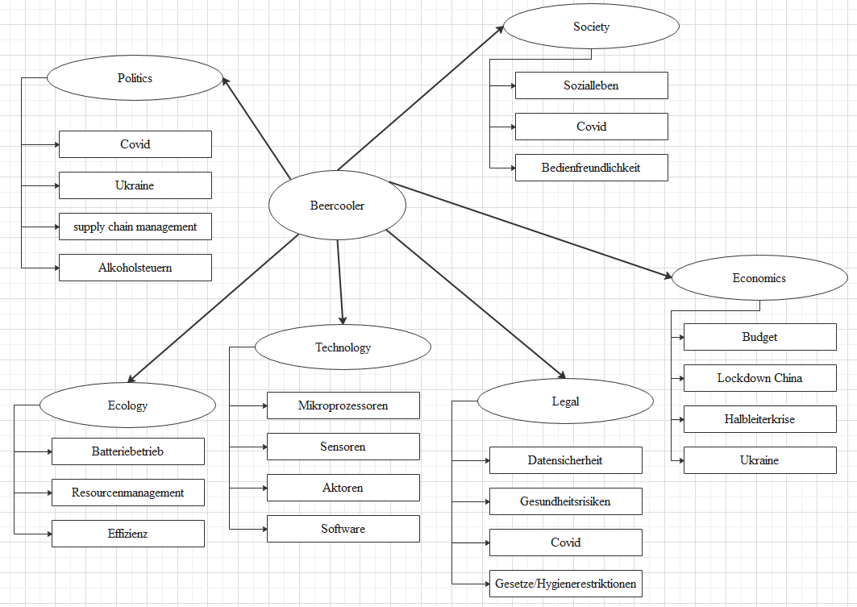
\includegraphics[width=\linewidth]{graphics/pestel.png}
\end{center}
\caption{Umfeld der Systemabgrenzung nach PESTEL}
\label{fig:pestel}
\end{figure}

\pagebreak

Das Eingriff System (Abbildung~\ref{fig:systemabgrenzung}) mit Umsystem hingegen 
vermittelt bereits ein deutlich klareres Bild.

\begin{figure}[h]
\begin{center}
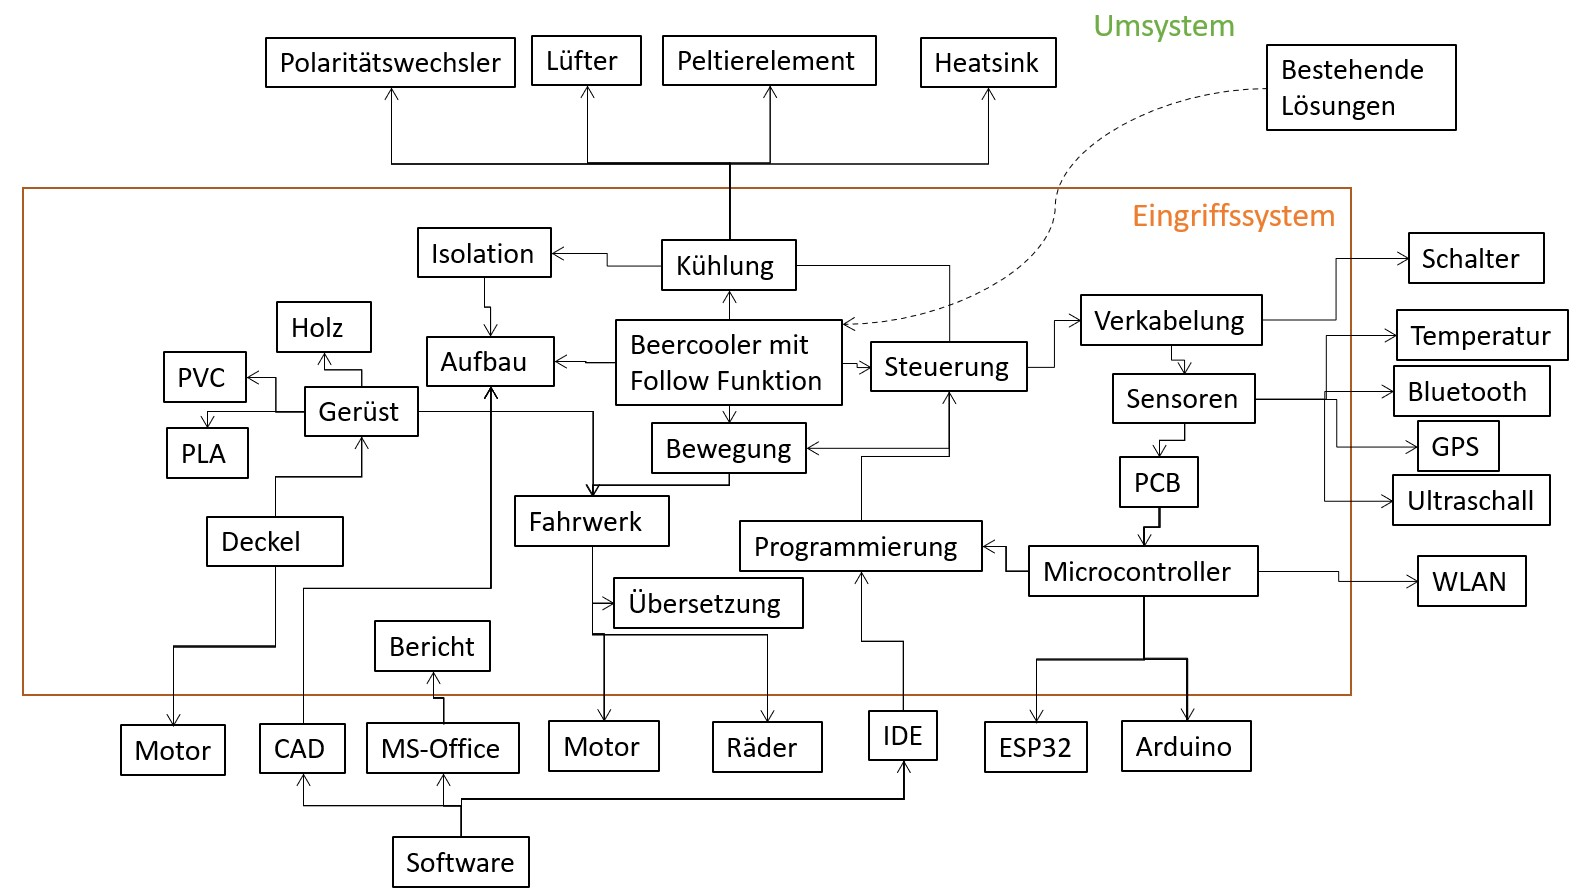
\includegraphics[width=\linewidth]{graphics/systemabgrenzung.jpg}
\end{center}
\caption{Umfeld der Systemabgrenzung nach PESTEL}
\label{fig:systemabgrenzung}
\end{figure}

\subsection{Zielkatalog}

Der Zielkatalog beschreibt unsere Anforderungen an das Projekt. Level 1 sind 
hierbei Ziele, die unbedingt erfüllt sein müssen, während Level 2 und 3 
Ausbaustufen darstellen, die weniger stark priorisiert werden. Zusammengefasst 
soll der Roboter also in der Lage sein, autonom einer Person zu folgen, 
mindestens ein Dutzend Bier zu beinhalten und diese über eine gewisse Zeit 
aktiv zu kühlen.

\textbf{Zielkatalog Level 1}



\textbf{Zielkatalog Level 2}



\textbf{Zielkatalog Level 3}

